\begin{figure}[t!]
    \centering
    \begin{subfigure}[t]{0.31\textwidth}
    \centering
    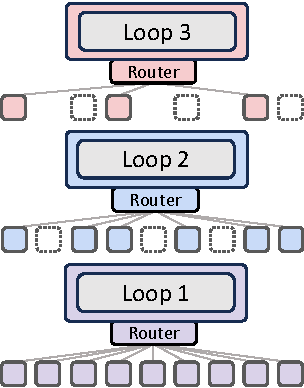
\includegraphics[width=0.7\textwidth]{figs/overview/method_expert_choice.pdf}
        \centering
        \captionsetup{justification=centering}
        \subcaption{Expert-choice routing}
        \label{fig:method_overview-a}
    \end{subfigure}
    \hfill
    \begin{subfigure}[t]{0.41\textwidth}
    \centering
    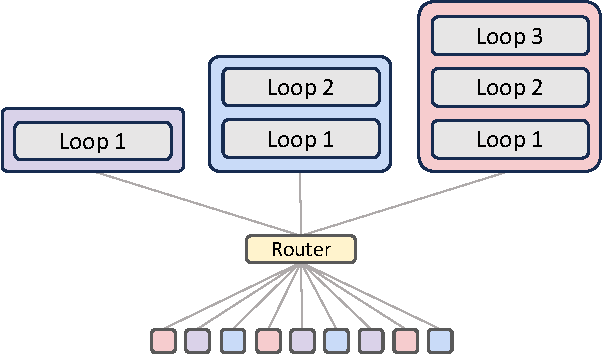
\includegraphics[width=\textwidth]{figs/overview/method_token_choice.pdf}
        \centering
        \captionsetup{justification=centering}
        \subcaption{Token-choice routing}
        \label{fig:method_overview-b}
    \end{subfigure}
    \centering
    \hfill
    \begin{subfigure}[t]{0.245\textwidth}
        \centering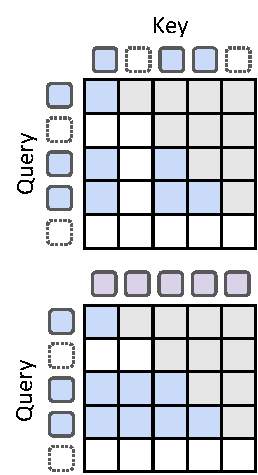
\includegraphics[width=0.65\textwidth]{figs/overview/method_caching.pdf}
        \captionsetup{justification=centering}
        \subcaption{Caching mechanism}
        \label{fig:method_overview-c}
    \end{subfigure}
    \caption{
        Architectural components of Mixture-of-Recursions (MoR).  
        (\textit{a}) {Expert-choice routing:} At each recursion step, a router selects top-$k$ tokens to continue, progressively narrowing the set of active tokens with depth.  
        (\textit{b}) {Token-choice routing:} Each token is assigned a fixed recursion step at the outset via a single routing decision, defining its complete compute path through the model.  
        (\textit{c}) {KV caching strategies:} Each square in the matrix represents whether a token (row) attends to another token’s cached key (column).  
        In ``recursion-wise KV caching'' (\textit{Top}), only the keys of currently selected (non-dropped) tokens at each recursion step are cached (\raisebox{0pt}[0.1em][0.1em]{\colorbox{custom_blue}{blue}}), and attention is restricted only to these entries.  
        In ``recursive KV sharing'' (\textit{Bottom}), all keys of previous tokens are cached at the first recursion step (\raisebox{0pt}[0.1em][0.1em]{\colorbox{custom_purple}{purple}}) and shared across subsequent recursion steps for attention operations.\looseness=-1
        }
    \label{fig:method_overview}
\end{figure}